\documentclass[tikz,border=8pt]{standalone}
\usepackage{amsmath}
\usetikzlibrary{arrows.meta}
\begin{document}
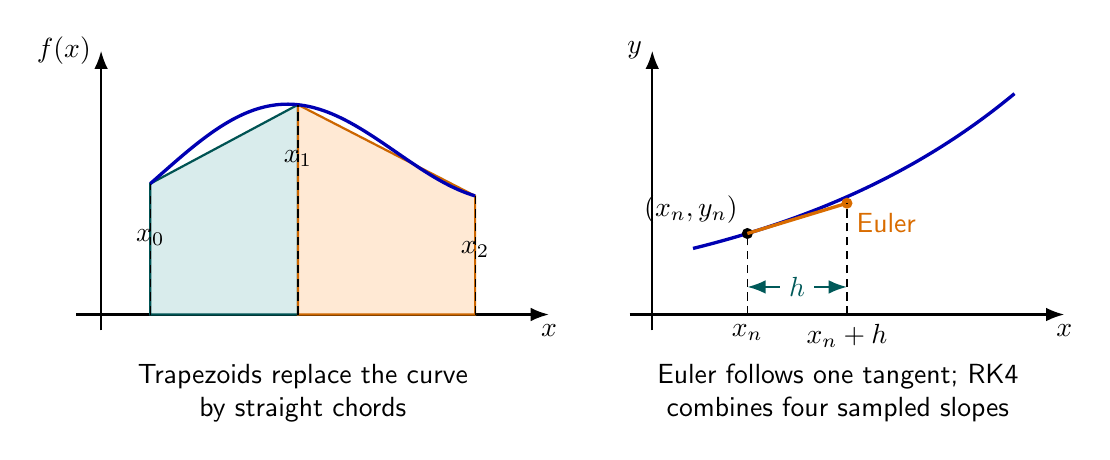
\begin{tikzpicture}[>=Latex,font=\sffamily]
\begin{scope}[x=1.25cm,y=1.0cm]
  \draw[->,thick] (-.25,0)--(4.55,0) node[below] {$x$};
  \draw[->,thick] (0,-.2)--(0,3.35) node[left] {$f(x)$};
  \pgfmathsetmacro{\xzero}{0.5}
  \pgfmathsetmacro{\xone}{2.0}
  \pgfmathsetmacro{\xtwo}{3.8}
  \pgfmathsetmacro{\yzero}{1.7+0.75*sin(75*(\xzero-.6))+0.12*\xzero}
  \pgfmathsetmacro{\yone}{1.7+0.75*sin(75*(\xone-.6))+0.12*\xone}
  \pgfmathsetmacro{\ytwo}{1.7+0.75*sin(75*(\xtwo-.6))+0.12*\xtwo}
  \draw[fill=teal!15,draw=teal!65!black,thick]
    (\xzero,0)--(\xzero,\yzero)--(\xone,\yone)--(\xone,0)--cycle;
  \draw[fill=orange!17,draw=orange!80!black,thick]
    (\xone,0)--(\xone,\yone)--(\xtwo,\ytwo)--(\xtwo,0)--cycle;
  \draw[very thick,blue!70!black,domain=.5:3.8,samples=100]
    plot (\x,{1.7+0.75*sin(75*(\x-.6))+0.12*\x});
  \draw[densely dashed] (\xzero,0)--(\xzero,\yzero)
    node[below=13pt] {$x_0$};
  \draw[densely dashed] (\xone,0)--(\xone,\yone)
    node[below=13pt] {$x_1$};
  \draw[densely dashed] (\xtwo,0)--(\xtwo,\ytwo)
    node[below=13pt] {$x_2$};
  \node[align=center] at (2.05,-1.0) {Trapezoids replace the curve\\by straight chords};
\end{scope}
\begin{scope}[xshift=7.0cm,x=1.15cm,y=1.0cm]
  \draw[->,thick] (-.25,0)--(4.55,0) node[below] {$x$};
  \draw[->,thick] (0,-.2)--(0,3.35) node[left] {$y$};
  \draw[very thick,blue!70!black,domain=.45:4.0,samples=100] plot (\x,{0.72*exp(0.34*\x)});
  \pgfmathsetmacro{\xn}{1.05}
  \pgfmathsetmacro{\hstep}{1.10}
  \pgfmathsetmacro{\yn}{0.72*exp(0.34*\xn)}
  \pgfmathsetmacro{\yeuler}{\yn+\hstep*0.34*\yn}
  \coordinate (P) at (\xn,\yn);
  \coordinate (Q) at ({\xn+\hstep},\yeuler);
  \fill (P) circle (2pt) node[above left] {$(x_n,y_n)$};
  \fill[orange!85!black] (Q) circle (2pt) node[below right] {Euler};
  \draw[orange!85!black,very thick] (P)--(Q);
  \draw[densely dashed] (\xn,0) node[below] {$x_n$}--(P);
  \draw[densely dashed] ({\xn+\hstep},0) node[below] {$x_n+h$}--(Q);
  \draw[<->,teal!70!black,thick] (\xn,.35)--({\xn+\hstep},.35)
    node[midway,fill=white] {$h$};
  \node[align=center] at (2.05,-1.0) {Euler follows one tangent; RK4\\combines four sampled slopes};
\end{scope}
\end{tikzpicture}
\end{document}
